\documentclass[tikz]{standalone}
\input{../standalonepreamble.tex}
\usetikzlibrary{shapes.misc}

\tikzset{nonterminal/.style={
  % The shape:
  rectangle,
  % The size:
  minimum size=6mm,
  % The border:
  very thick,
  draw=red!50!black!50,
  % The filling:
  top color=white,
  bottom color=red!50!black!20,
  % Font:
  font=\itshape,
  }
}

\tikzset{terminal/.style={
  % The shape:
  rounded rectangle,
  minimum size=6mm,
  % The rest
  very thick,draw=black!50,
  top color=white,bottom color=black!20,
  font=\ttfamily,
  }
}



\begin{document}


\begin{tikzpicture}[node distance=5mm]
  \node [nonterminal] {unsigned integer};
\end{tikzpicture}

\begin{tikzpicture}[node distance=5mm,
        text height=1.5ex,text depth=0.25em
  ]
  \node (dot)   [terminal]                {.};
  \node (digit) [terminal,right=of dot]   {digit};
  \node (E)     [terminal,right=of digit] {E};
\end{tikzpicture}


\begin{tikzpicture}[
    node distance=5mm and 5mm,
    terminal/.append style={rectangle,rounded corners=3mm},
    skip loop/.style={to path={-- ++(0,#1) -| (\tikztotarget)}}
  ]
  \node (ui1)   [nonterminal]                      {unsigned integer};
  \node (dot)   [terminal,right=of ui1]            {.};
  \node (digit) [terminal,right=of dot]            {digit};
  \node (E)     [terminal,right=of digit]          {E};
  \node (plus)  [terminal,above right=of E]        {+};
  \node (minus) [terminal,below right=of E]        {-};
  \node (ui2)   [nonterminal,below right=of plus]  {unsigned integer};

  \path (dot)   edge[->]                   (digit)  % simple edges
        (digit) edge[->]                   (E)
        ($ (digit.east)!0.5!(E.west) $)
                edge[->,skip loop=-5mm] ($ (digit.west)!0.5!(dot.east) $);
\end{tikzpicture}


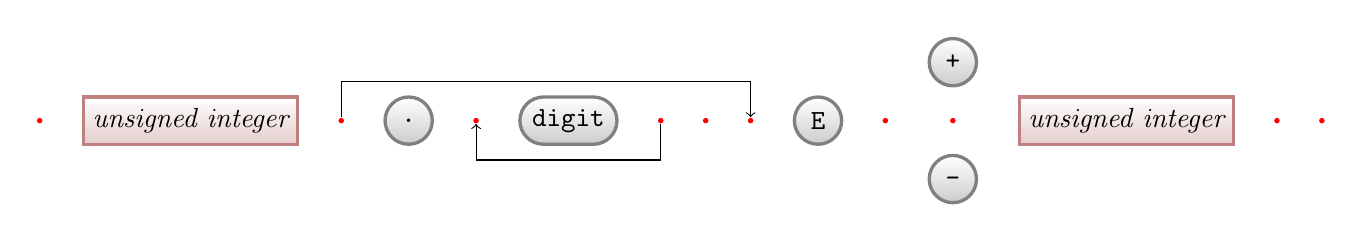
\begin{tikzpicture}[point/.style={circle,inner sep=0pt,minimum
        size=2pt,fill=red}, skip loop/.style={to path={-- ++(0,#1) -|
        (\tikztotarget)}}]
  \matrix[row sep=1mm,column sep=5mm] {
    % First row:
      & & & & & & & & & & & \node (plus) [terminal] {+}; \\
    % Second row:
    \node (p1) [point]  {}; &    \node (ui1)   [nonterminal] {unsigned integer}; &
    \node (p2) [point]  {}; &    \node (dot)   [terminal]    {.};                &
    \node (p3) [point]  {}; &    \node (digit) [terminal]    {digit};            &
    \node (p4) [point]  {}; &    \node (p5)    [point]  {}; &    
    \node (p6) [point]  {}; &    \node (e)     [terminal]    {E};                &
    \node (p7) [point]  {};                                                      &
    \node (p8) [point]  {}; &    \node (ui2)   [nonterminal] {unsigned integer}; & 
    \node (p9) [point]  {}; &    \node (p10)   [point]       {};\\
    % Third row:
    & & & & & & & & & & & \node (minus) [terminal] {-};\\
  };

  \path (p4) edge [->,skip loop=-5mm] (p3)
        (p2) edge [->,skip loop=5mm]  (p6);
\end{tikzpicture}

\end{document}
